\documentclass{beamer}
\usepackage{graphicx}
\usepackage{amsfonts}
\usepackage{amssymb}
\usepackage{amsthm}
\usepackage{mathtools}
\usepackage{mathrsfs}
\usepackage{tikz}
\usepackage{graphtheory}

\renewcommand{\P}{\mathcal{P}}
\newcommand{\txtclr}[1]{\textcolor{#1}{#1}}  % colored text
\newcommand{\mtxtclr}[1]{\text{\txtclr{#1}}}  % colored text in math mode
\renewcommand{\a}{\alpha}
\newcommand{\w}{\omega}
\newcommand{\X}{\chi}
\DeclarePairedDelimiter{\abs}{\lvert}{\rvert}
\DeclarePairedDelimiter{\set}{\{}{\}}

\title{Determining a Graph's Chromatic Number for Part Consolidation in Axiomatic Design}
\author{Jeffery A. Cavallaro}
\institute{San Jose State University \\ Department of Mathematics}
\date{27 March 2020}

\begin{document}

\frame{\titlepage}

\begin{frame}
  \frametitle{Axiomatic Design}
  \begin{itemize}
  \item Formalizes the design process without affecting creativity.
  \item Attempts to identify those traits common to successful designs.
  \item Starts with a set of \emph{functional requirements} (FRs) that address customer needs.
  \item Designers construct \emph{design parameters} (DPs) to satisfy the FRs.
  \item Provides a framework for comparing different designs.
  \end{itemize}
\end{frame}

\begin{frame}
  \frametitle{The Axioms}
  \begin{block}{The Independence Axiom}
    An optimal design always maintains the independence of the FRs. This means that the FRs and DPs are related in
    such a way that a specific DP can be adjusted to satisfy its corresponding FR without affecting other FRs.
  \end{block}
  \begin{block}{The Information Axiom}
    The best design is a functionally uncoupled design that has the minimum information content.
  \end{block}
\end{frame}

\begin{frame}
  \frametitle{Part Consolidation}
  \begin{itemize}
  \item Minimize information content by consolidating multiple FRs and their DPs into a single part.
  \item The minimum number of parts needed to satisfy all FRs is a key metric for comparing designs.
  \item Opener example: 2 FRs (open bottles, open cans) and 1 part.
  \end{itemize}

  \begin{center}
    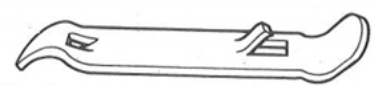
\includegraphics[scale=0.5]{opener}
  \end{center}
\end{frame}

\begin{frame}
  \frametitle{A Graph Theory Solution}
  \begin{itemize}
  \item Let the FRs be vertices in a simple graph.
  \item If two FRs cannot be combined into the same part for some reason then add an edge between their vertices.
  \item The minimum number of parts problem becomes a chromatic coloring problem of the resulting graph.
  \end{itemize}
\end{frame}

\begin{frame}
  \frametitle{The Chromatic Coloring Problem}
  \begin{itemize}
  \item Inherently intractable (steps/time required to solve increases exponentially with order, NP-hard).
  \item P-time algorithms to estimate: not exact but maybe a good start.
  \item Exact algorithms:
    \begin{itemize}
    \item Christofides
    \item Zykov
    \item Jahanbekam/Cavallaro (proposed by this research)
    \end{itemize}
  \item Solution Parameters:
    \begin{itemize}
    \item Approximately 20 FRs (vertices).
    \item Moderate edge density.
    \item Runtime duration of under one minute.
    \end{itemize}
  \end{itemize}
\end{frame}

\begin{frame}
  \frametitle{Simple Graphs}
  \begin{itemize}
  \item A mathematical object \(G=(V,E)\) that includes a set of vertices (nodes) \(V(G)\) and and set of edges
    \(E(G)\).
  \item Each edge is a 2-element subset of \(V(G)\): \(E(G)\subset\P_2(V(G))\).
  \item Edges are identified by juxtaposition: \(\set{a,b}=ab=ba\).
  \item No multiple edges and no loops.
  \item Vertices can be labeled or unlabeled.
  \end{itemize}
\end{frame}

\begin{frame}
  \frametitle{Simple Graph Example}
  \begin{center}
    \begin{minipage}{2in}
      \vspace{0in}
      \centering
      \begin{tikzpicture}[node distance=1cm,every node/.style={labeled node}]
        \node (E) at (0,0) {\(e\)};
        \node (A) [above left=of E] {\(a\)};
        \node (B) [above right=of E] {\(b\)};
        \node (C) [below right=of E] {\(c\)};
        \node (D) [below left=of E] {\(d\)};
        \draw (A) edge (B);
        \draw (B) edge (E);
        \draw (E) edge (A);
        \draw (A) edge (D);
      \end{tikzpicture}

      \bigskip

      LABELED
    \end{minipage}
    \begin{minipage}{2in}
      \vspace{0in}
      \centering
      \begin{tikzpicture}[node distance=1.75cm,every node/.style={unlabeled node}]
        \node (E) at (0,0) {};
        \node (A) [above left=of E] {};
        \node (B) [above right=of E] {};
        \node (C) [below right=of E] {};
        \node (D) [below left=of E] {};
        \draw (A) edge (B);
        \draw (B) edge (E);
        \draw (E) edge (A);
        \draw (A) edge (D);
      \end{tikzpicture}

      \bigskip

      UNLABELED
    \end{minipage}
    \begin{gather*}
      V(G)=\set{a,b,c,d,e} \\
      E(G)=\set[\big]{ab,ad,ae,be}
    \end{gather*}
  \end{center}
\end{frame}

\begin{frame}
  \frametitle{Adjacent Vertices}
  \begin{itemize}
  \item Vertices joined by an edge are \emph{adjacent} or \emph{neighbors}.
  \item An edge \emph{joins} and is \emph{incident} to its vertices.
  \item An \emph{isolated} vertex has no neighbors.
  \end{itemize}
\end{frame}

\begin{frame}
  \frametitle{Order and Size}
  \begin{itemize}
  \item The \emph{order} of a graph is the number of vertices: \(n=\abs{V(G)}\).
  \item The \emph{size} of a graph is the number of edges: \(m=\abs{E(G)}\).
  \item \(\displaystyle m\le\binom{n}{2}=\frac{n(n-1)}{2}\)
  \end{itemize}
\end{frame}

\begin{frame}
  \frametitle{Order/Size Special Cases}
  \begin{itemize}
  \item The \emph{null} graph has no vertices (\(n=m=0\)).
  \item An \emph{empty} graph has no edges (m=0).
  \item A \emph{complete} graph has every possible edge \(\displaystyle\left(m=\frac{n(n-1)}{2}\right)\).
  \end{itemize}
\end{frame}

\begin{frame}
  \frametitle{Graph Coloring}
  \begin{itemize}
  \item A \emph{coloring} of a graph is a function \(c:V(G)\to C\) that assigns a color from \(C\) to each vertex.
  \item A \emph{proper} coloring of a graph assigns different colors to adjacent vertices:
    \(uv\in E(G)\implies c(u)\ne c(v)\).
  \item The coloring function need not be surjective.
  \item A proper coloring with \(\abs{C}=k\) is called a \(k\)-coloring.
  \item A \(k\)-colorable graph is also \((k+1)\)-colorable.
  \item If \(n\le k\) then a graph is guaranteed to be \(k\)-colorable.
  \item A coloring for a minimum \(k\) is called a \emph{chromatic} coloring.
  \item The minimum such \(k\) is called the \emph{chromatic number} of a graph: \(\X(G)\).
  \end{itemize}
\end{frame}

\begin{frame}
  \frametitle{\(4\)-coloring Example}
  \begin{minipage}{2in}
    \centering
    \begin{tikzpicture}
      \colorlet{c1}{green!50!white}
      \colorlet{c2}{blue!50!white}
      \colorlet{c3}{red!50!white}
      \colorlet{c4}{orange!50!white}
      \begin{scope}[node distance=1cm,every node/.style={labeled node}]
        \node (E) [fill=c3] at (0,0) {\(e\)};
        \node (A) [above left=of E,fill=c1] {\(a\)};
        \node (B) [above right=of E,fill=c2] {\(b\)};
        \node (C) [below right=of E,fill=c1] {\(c\)};
        \node (D) [below left=of E,fill=c4] {\(d\)};
      \end{scope}
      \draw (A) edge (B);
      \draw (B) edge (E);
      \draw (E) edge (A);
      \draw (A) edge (D);
      \draw (E) edge (C);
    \end{tikzpicture}
  \end{minipage}
  \begin{minipage}{2in}
    \centering
    \(C=\set{\mtxtclr{green},\mtxtclr{blue},\mtxtclr{red},\mtxtclr{orange}}\)
    \begin{align*}
      c(a) &= \mtxtclr{green} \\
      c(b) &= \mtxtclr{blue} \\
      c(c) &= \mtxtclr{green} \\
      c(d) &= \mtxtclr{orange} \\
      c(e) &= \mtxtclr{red}
    \end{align*}
  \end{minipage}
\end{frame}

\begin{frame}
  \frametitle{\(5\)-coloring Example}
  \begin{minipage}{2in}
    \centering
    \begin{tikzpicture}
      \colorlet{c1}{green!50!white}
      \colorlet{c2}{blue!50!white}
      \colorlet{c3}{red!50!white}
      \colorlet{c4}{orange!50!white}
      \begin{scope}[node distance=1cm,every node/.style={labeled node}]
        \node (E) [fill=c3] at (0,0) {\(e\)};
        \node (A) [above left=of E,fill=c1] {\(a\)};
        \node (B) [above right=of E,fill=c2] {\(b\)};
        \node (C) [below right=of E,fill=c1] {\(c\)};
        \node (D) [below left=of E,fill=c4] {\(d\)};
      \end{scope}
      \draw (A) edge (B);
      \draw (B) edge (E);
      \draw (E) edge (A);
      \draw (A) edge (D);
      \draw (E) edge (C);
    \end{tikzpicture}
  \end{minipage}
  \begin{minipage}{2.2in}
    \centering
    \scalebox{0.9}{
      \(C=\set{\mtxtclr{green},\mtxtclr{blue},\mtxtclr{red},\mtxtclr{orange},\mtxtclr{brown}}\)
    }
    \begin{align*}
      c(a) &= \mtxtclr{green} \\
      c(b) &= \mtxtclr{blue} \\
      c(c) &= \mtxtclr{green} \\
      c(d) &= \mtxtclr{orange} \\
      c(e) &= \mtxtclr{red} \\
    \end{align*}
  \end{minipage}
\end{frame}

\begin{frame}
  \frametitle{Chromatic Coloring Example}
  \begin{minipage}{2in}
    \centering
    \begin{tikzpicture}
      \colorlet{c1}{green!50!white}
      \colorlet{c2}{blue!50!white}
      \colorlet{c3}{red!50!white}
      \begin{scope}[node distance=1cm,every node/.style={labeled node}]
        \node (E) [fill=c3] at (0,0) {\(e\)};
        \node (A) [above left=of E,fill=c1] {\(a\)};
        \node (B) [above right=of E,fill=c2] {\(b\)};
        \node (C) [below right=of E,fill=c1] {\(c\)};
        \node (D) [below left=of E,fill=c2] {\(d\)};
      \end{scope}
      \draw (A) edge (B);
      \draw (B) edge (E);
      \draw (E) edge (A);
      \draw (A) edge (D);
      \draw (E) edge (C);
    \end{tikzpicture}
  \end{minipage}
  \begin{minipage}{2in}
    \[C=\set{\mtxtclr{green},\mtxtclr{blue},\mtxtclr{red}}\]
    \begin{align*}
      c(a) &= \mtxtclr{green} \\
      c(b) &= \mtxtclr{blue} \\
      c(c) &= \mtxtclr{green} \\
      c(d) &= \mtxtclr{blue} \\
      c(e) &= \mtxtclr{red}
    \end{align*}
  \end{minipage}
\end{frame}

\begin{frame}
  \frametitle{Mutators: Vertex Removal}
  \begin{itemize}
  \item Removes one or more vertices (and their incident edges).
  \end{itemize}

  \bigskip

  \begin{center}
    \begin{minipage}{2in}
      \centering
      \begin{tikzpicture}[node distance=0.75cm,every node/.style={labeled node}]
        \node [red] (E) at (0,0) {\(e\)};
        \node (A) [above left=of E] {\(a\)};
        \node (B) [above right=of E] {\(b\)};
        \node [red] (C) [below right=of E] {\(c\)};
        \node (D) [below left=of E] {\(d\)};
        \draw (A) edge (B);
        \draw [red] (B) edge (E);
        \draw [red] (E) edge (A);
        \draw (A) edge (D);
      \end{tikzpicture}

      \bigskip

      \(G\)
    \end{minipage}
    \begin{minipage}{2in}
      \centering
      \begin{tikzpicture}[node distance=0.75cm,every node/.style={labeled node}]
        \node (A) [above left=of E] {\(a\)};
        \node (B) [above right=of E] {\(b\)};
        \node (C) [below right=of E,white] {\(c\)};
        \node (D) [below left=of E] {\(d\)};
        \draw (A) edge (B);
        \draw (A) edge (D);
      \end{tikzpicture}

      \bigskip

      \(G-\set{c,e}\)
    \end{minipage}
  \end{center}
\end{frame}

\begin{frame}
  \frametitle{Mutators: Edge Addition}
  \begin{itemize}
  \item Adds an edge between two non-adjacent vertices.
  \item Vertices are forced to have different colors in a proper coloring.
  \end{itemize}

  \bigskip

  \begin{center}
    \begin{minipage}{2in}
      \centering
      \begin{tikzpicture}[node distance=0.75cm,every node/.style={labeled node}]
        \node (E) at (0,0) {\(e\)};
        \node (A) [above left=of E] {\(a\)};
        \node (B) [above right=of E] {\(b\)};
        \node (C) [below right=of E] {\(c\)};
        \node (D) [below left=of E] {\(d\)};
        \draw (A) edge (B);
        \draw (B) edge (E);
        \draw (E) edge (A);
        \draw (A) edge (D);
      \end{tikzpicture}

      \bigskip

      \(G\)
    \end{minipage}
    \begin{minipage}{2in}
      \centering
      \begin{tikzpicture}[node distance=0.75cm,every node/.style={labeled node}]
        \node (E) at (0,0) {\(e\)};
        \node (A) [above left=of E] {\(a\)};
        \node (B) [above right=of E] {\(b\)};
        \node (C) [below right=of E] {\(c\)};
        \node (D) [below left=of E] {\(d\)};
        \draw (A) edge (B);
        \draw (B) edge (E);
        \draw (E) edge (A);
        \draw (A) edge (D);
        \draw [green] (C) edge (D);
      \end{tikzpicture}

      \bigskip

      \(G+cd\)
    \end{minipage}
  \end{center}
\end{frame}

\begin{frame}
  \frametitle{Mutators: Vertex Contraction}
  \begin{itemize}
  \item Two vertices are identified as one.
  \item Any edge between the two vertices is discarded.
  \item Resulting multiple edges are reduced to a single edge.
  \end{itemize}

  \bigskip

  \begin{center}
    \begin{minipage}{2in}
      \centering
      \begin{tikzpicture}[scale=0.5,every node/.style={labeled node}]
        \cycleVnodes{\(a\),\(b\),\(c\),\(d\),\(e\)}{(0,0)}{1in}{90}{}
        \draw (1) edge (5);
        \draw (2) edge (3) edge (4) edge (5);
        \draw (3) edge (4);
        \draw (4) edge (5);
        \draw [dashed,red,->] (2) edge (1);
      \end{tikzpicture}

      \bigskip

      \(G\)
    \end{minipage}
    \begin{minipage}{2in}
      \centering
      \begin{tikzpicture}[scale=0.5]
        \begin{scope}[every node/.style={coordinate}]
          \cycleNnodes{5}{(0,0)}{1in}{90}{}
        \end{scope}
        \begin{scope}[every node/.style={labeled node}]
          \node (AB) at (1) {\(ab\)};
          \node (C) at (3) {\(c\)};
          \node (D) at (4) {\(d\)};
          \node (E) at (5) {\(e\)};
        \end{scope}
        \draw (AB) edge (C) edge (D) edge (E);
        \draw (C) edge (D);
        \draw (D) edge (E);
      \end{tikzpicture}

      \bigskip

      \(G\cdot ab\)
    \end{minipage}
  \end{center}
\end{frame}

\begin{frame}
  \frametitle{Mutators: Complement}
  \begin{itemize}
  \item Adjacent vertices in \(G\) are not adjacent in \(\bar{G}\), and vice versa:
    \[uv\in E(G)\iff uv\notin E(\bar{G})\]
  \end{itemize}

  \bigskip

  \begin{center}
    \begin{minipage}{2in}
      \centering
      \begin{tikzpicture}[scale=0.5,every node/.style={labeled node}]
        \cycleVnodes{\(a\),\(b\),\(c\),\(d\)}{(0,0)}{0.75in}{135}{};
        \draw (1) edge (2) edge (3) edge (4);
        \draw [red, dashed] (2) edge (3);
        \draw [red, dashed] (2) edge (4);
        \draw [red, dashed] (3) edge (4);
      \end{tikzpicture}

      \bigskip

      \(G\)
    \end{minipage}
    \begin{minipage}{2in}
      \centering
      \begin{tikzpicture}[scale=0.5,every node/.style={labeled node}]
        \cycleVnodes{\(a\),\(b\),\(c\),\(d\)}{(0,0)}{0.75in}{135}{};
        \draw [red, dashed] (1) edge (2) edge (3) edge (4);
        \draw (2) edge (3);
        \draw (2) edge (4);
        \draw (3) edge (4);
      \end{tikzpicture}

      \bigskip

      \(\bar{G}\)
    \end{minipage}
  \end{center}
\end{frame}

\begin{frame}
  \frametitle{Independent (Stable) Sets}
  \begin{itemize}
  \item A subset of \(V(G)\) whose elements are nonadjacent vertices.
  \item Maximal (MIS) if not a proper subset of some other independent set.
  \item Maximum if cardinality is \(\ge\) any other MIS.
  \item The \emph{independence number} \(\a(G)\) is the cardinality of a maximum MIS in \(G\).
  \item A proper coloring distributes vertices into independent sets.
  \item A chromatic coloring partitions vertices into independent sets.
  \end{itemize}
\end{frame}

\begin{frame}
  \frametitle{MIS Example}
  \begin{center}
    \begin{minipage}{2in}
      \centering
      \begin{tikzpicture}[scale=0.7,every node/.style={labeled node}]
        \node (a) at (0,0) {\(a\)};
        \node (b) at (2,0) {\(b\)};
        \node (c) at (4,0) {\(c\)};
        \node (d) at (6,0) {\(d\)};
        \node (e) at (5,-2) {\(e\)};
        \node (f) at (3,-2) {\(f\)};
        \node (g) at (1,-2) {\(g\)};
        \node (h) at (3,2) {\(h\)};
        \draw (a) edge (f) edge (g) edge (h);
        \draw (b) edge (f) edge (h);
        \draw (c) edge (e) edge (f) edge (h);
        \draw (d) edge (e) edge (f) edge (h);
      \end{tikzpicture}
    \end{minipage}
    \begin{minipage}{2in}
      \centering
      \begin{tabular}{c|c}
        MIS & SIZE \\
        \hline
        \(\set{a, b, c, d}\) & \(4\) \\
        \(\set{a, b, e}\) & \(3\) \\
        \(\set{b, c, d, g}\) & \(4\) \\
        \(\set{b, e, g}\) & \(3\) \\
        \(\set{e, f, g, h}\) & \(4\)
      \end{tabular}

      \bigskip

      \(\a(G)=4\)
    \end{minipage}
  \end{center}
\end{frame}

\begin{frame}
  \frametitle{Cliques}
  \begin{itemize}
  \item A complete graph embedded in (a subgraph of) a graph.
  \item A clique of order \(k\) is called a \(k\)-clique.
  \item A proper coloring for a graph with a \(k\)-clique requires at least \(k\) colors.
  \item Maximal if not a subgraph some other clique.
  \item Maximum if order is \(\ge\) any other clique.
  \item The \emph{clique number} \(\w(G)\) is the order of a max clique in \(G\).
  \item A (maximal) clique in \(G\) is a (maximal) independent set in \(\bar{G}\).
  \end{itemize}
\end{frame}

\begin{frame}
  \frametitle{Maximal Clique Example}
  \begin{center}
    \begin{minipage}{3.5in}
      \centering
      \scalebox{0.75}{
        \begin{tikzpicture}[every node/.style=labeled node]
          \completeV{\(a\),\(b\),\(c\),\(d\)}{(0,0)}{0.75in}{135}{a};
          \completeV{\(e\),\(f\),\(g\)}{(5,0)}{0.6in}{120}{b};
          \node (h) [right=of b2] {\(h\)};
          \draw (a2) edge (b1);
          \draw (a3) edge (b3);
          \draw (b2) edge (h);
          \draw (a1) -- ($(a1)+(0,1cm)$) -| (b1);
          \draw (a4) -- ($(a4)-(0,1cm)$) -| (b3);
          \draw (a2) -- (b3);
          \draw (b1) -| (h);
          \draw (b3) -| (h);
        \end{tikzpicture}
      }

      \(G\)
    \end{minipage}

    \bigskip

    \begin{minipage}{2in}
      \centering
      \scalebox{0.75}{
        \begin{tabular}{c|c}
          MAXIMAL CLIQUE & ORDER \\
          \hline
          \(G[\set{a, b, c, d}]\) & \(4\) \\
          \(G[\set{a, b, e}]\) & \(3\) \\
          \(G[\set{b, c, d, g}]\) & \(4\) \\
          \(G[\set{b, e, g}]\) & \(3\) \\
          \(G[\set{e, f, g, h}]\) & \(4\)
        \end{tabular}
      }
    \end{minipage}
    \begin{minipage}{1in}
      \(\w(G)=4\)
    \end{minipage}
  \end{center}
\end{frame}

\begin{frame}
  \frametitle{}
  \begin{itemize}
  \item
  \end{itemize}
\end{frame}

\end{document}
